\subsection{Corpus overview}
\label{subsec:data-overview}

\begin{figure}[t]
\centering
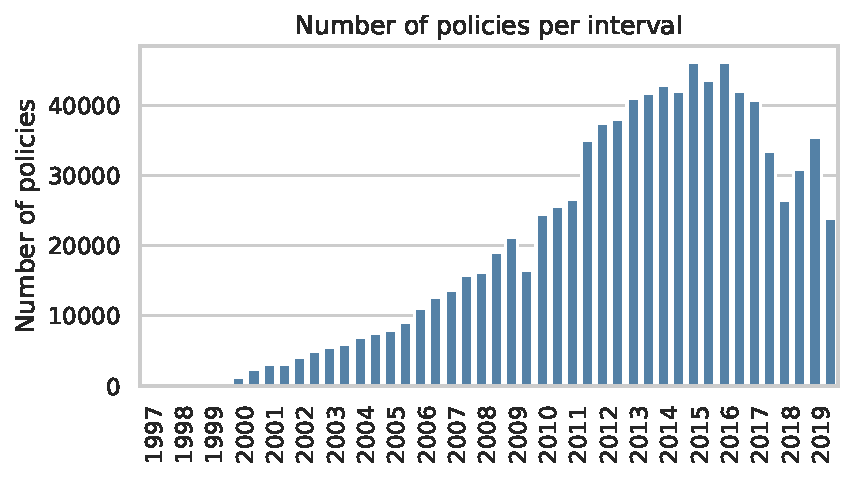
\includegraphics[width=0.99\columnwidth]{figures/policy_counts.pdf}
\caption{The number of privacy policies for each interval. Note that there are two intervals per year.}
\label{fig:numpolicies}
\end{figure}

Our dataset contains 1,0714,88 policies from 130,620 different websites.
Although the dataset contains policies from as early as 1997, 80.8\% of the policies are from snapshots archived in 2010 or later.
% we can use the following to justify the range we use for the trend plots [2000,2019]
% 99.92 of the policies are from 2000 or later
%There are $333987$ distinct policy texts, which indicates that many policies share a common text.

%In order to understand the scale of our dataset, w
We illustrate the number of privacy policies per six-month intervals in Figure~\ref{fig:numpolicies}.
The number of policies per interval increases almost every year until 2016, after which it declines. This pattern of policies per interval roughly follows the number of homepage snapshots we are able to access in that interval. \rnote{Should we maybe do this as a stacked bar graph? Or remove this last sentence?}
Recall that Alexa ranks are only available from 2009 onwards and we attempt to download policies from websites that were ever ranked in the Alexa top 100K (i.e. between 2009 and 2019).
The decreases in the number of policies in 2009B and 2018A also occur in the number of snapshots available on the Wayback Machine in those intervals, indicating that these decreases may be due to changes in archiving or incomplete archives for those intervals.

Only 5,138 (0.47\%) of the policies are of type PDF, whereas the remaining 1,066,350 are regular HTML pages.


% say more based on data or this discussion: https://princetoncitp.slack.com/archives/GTGC8NB18/p1586384536234100

% word count

% number of policies

% number of policies vs number of homepages

% categories